
%----------------------------------------------------------------------------------
%----Präambel/Preamble-------------------------------------------------------------
%----------------------------------------------------------------------------------

\documentclass[	a4paper,
				11pt,
				DIV=11,
				bigheadings,
				idxtotoc,
				listof=totoc,	
				bibtotoc,		
				halfparskip,
				cleardoubleempty,
				oneside,
				openright]{scrartcl}
%----------------------------------------------------------------------------------

\usepackage[english]{babel}
\usepackage[T1]{fontenc}
\usepackage[utf8]{inputenc}

\usepackage[OT1]{fontenc}
\renewcommand*\familydefault{\sfdefault}


\usepackage{graphicx}	

\usepackage[labelfont=bf]{caption}
					
\usepackage{float}
\usepackage{wrapfig}
%\usepackage{subfigure}

\usepackage{geometry}						% Für newgeometry in Titelseite
\geometry{a4paper,left=30mm,right=20mm}

\usepackage{blindtext}
\usepackage{layout}

\PassOptionsToPackage{hyphens}{url}		
\usepackage[pdfborder={0 0 0},
			colorlinks=true, 
			linkcolor=black,
			citecolor=red,
			]{hyperref}
			
\usepackage{natbib}%numbers 				

\usepackage{pdfpages}

\usepackage{color}
\usepackage{xcolor}

\usepackage{setspace}

\usepackage{longtable}
\usepackage{multirow}
\usepackage{colortbl}

%----------------------------------------------------------------------------------
%----Kopfzeile---------------------------------------------------------------------
%----------------------------------------------------------------------------------

\usepackage{scrlayer-scrpage} 							% Aufruf KOMA-Skript für Kopfzeilen

\pagestyle{scrheadings}							% Definition der Eigenen Headerformatierung
\clearscrheadfoot 								% alle Standard-Werte und Formatierungen raus
%\automark[chapter]{section}						% Kapitel und Section als Inhalt der Variablen leftmark und rightmark
\ohead{\pagemark}								% Seitenzahl auf äußerem Rand
\ihead{\ifthispageodd{\leftmark}{\rightmark}} 	% Innere Überschrift mit Kapitel bei linker Seite und Section bei rechter Seite -> geht nur in Verbindung mit
												% zweiseitigem Text wirklich sinnvoll
\setheadsepline{0.4pt} 							% Trennlinie Fußzeile und Textkörper
\setkomafont{pagehead}{\scshape}				% Schriftart in Kopfzeile, \scshape = Kapitelchen
%----Fußzeile----------------------------------------------------------------------
\setfootsepline{0.4pt} 							% Trennlinie Fußzeile und Textkörper
\setkomafont{pagefoot}{\scshape}				% Schriftart in Fußfzeile, \scshape = Kapitelchen
\ifoot{\footnotesize{John Doe}}
\ofoot{\footnotesize{Master thesis}}		
%----------------------------------------------------------------------------------

\defpagestyle{myPageStyle}{
	(0pt ,0pt)
	{\hfill\pagemark} {\hfill\pagemark} {\hfill\pagemark}
	(0pt ,0pt)	
}{
{
	(\textwidth ,0.4pt)
	\footnotesize{John Doe} \hfill \footnotesize{Master thesis}} 
	{\footnotesize{John Doe} \hfill \footnotesize{Master thesis}} 
	{\footnotesize{John Doe} \hfill \footnotesize{Master thesis}}
	(0pt ,0pt)
}


%----Farbdefinition--THI-blau------------------------------------------------------
\definecolor{haw_mag}{rgb}{0,0.112,0.47}
\addtokomafont{section}{\color{haw_mag} \rmfamily \scshape} 
\addtokomafont{subsection}{\color{haw_mag} \rmfamily}
\addtokomafont{subsubsection}{\color{haw_mag} \rmfamily}
\addtokomafont{paragraph}{\color{haw_mag} \rmfamily}
\addtokomafont{subparagraph}{\rmfamily}
%----------------------------------------------------------------------------------

\definecolor{tab_2}{RGB}{230,230,230}
\definecolor{tab_1}{RGB}{85,128,214}

%------Längenanpassung-------------------------------------------------------------
\setlength{\headsep}{10mm}						% Textabstand zur Kopfzeile
\setlength{\footskip}{15mm}						% Abstand zur Fußzeile
\setlength{\textheight}{235mm}					% Texthöhe
%----------------------------------------------------------------------------------


%----Glossar-----------------------------------------------------------------------
\usepackage[toc, acronym]{glossaries} 			
\makeglossaries	

%----------------------------------------------------------------------------------
%----Glossar-----------------------------------------------------------------------
\usepackage[intoc]{nomencl} 
\makenomenclature
%----------------------------------------------------------------------------------



\includeonly{	
	titlepage,							
	affidavit,
	acknowledgments,
	%abstractDE,
	abstractEN,
	confidentialityClause,
	glossary,
	mainpart,
	%outlook,
	%fazit,
	nomenclature,
	appendices
	}
	
			
%-------------------------------------------------------------------------------------------------------------------------------------------------------------
%----------------DOKUMENT-BEGINN---------------------------------------------------
%-------------------------------------------------------------------------------------------------------------------------------------------------------------

\begin{document}

	%\shorthandoff{"}						% Vermeidung von ungewollten Ligaturen/Avoid unwanted ligatures
	
	%----Vermeidung von Hurenkindern und Schusterjungen---------------------
	\widowpenalty=10000
	\clubpenalty=10000
	\displaywidowpenalty=10000	
	%-----------------------------------------------------------------------

	%Titelseite/title page	
	%----------Titelseite-------------------------------------------------------------

\newgeometry{textheight=0.9\paperheight, textwidth=0.76\paperwidth, left=30mm, right=20mm}

\begin{titlepage}	
	%----THI+(x-company)-logo--------------------------------------------------------
	\begin{figure}[!h]
		\centering
		    %---- Add Cooperation here and add scaling if necessary 
			
\includegraphics[width={0.2\textwidth}]{images/ai-motion.png}	
			\hfill
			
\includegraphics[width={0.1\textwidth}]{images/cvims_logo_dark.png}	
			\hfill
			
\includegraphics[width={0.2\textwidth}]{images/thiRGB.jpg}	
		\end{figure}																			
	%------------------------------------------------------------------------------
	
	\begin{center}
		\hrulefill 
	\end{center}
	
	
	\begin{center}	
		\vspace{1cm}
		\huge\textbf{Technische Hochschule Ingolstadt}\\[1em]
		\Large \textbf{Faculty of Computer Science}\\ 
		\normalsize
		Computer Vision for Intelligent Mobility Systems \\ 
		Study Program Computer Science - Security and Safety \\ [2.5em]
	\end{center}


	\begin{center}	
		\vspace{1cm}
		\Large \textbf{Master Thesis}\\ 
		\normalsize
		for the degree of \\ 
		Master of Science (M. Sc.) \\ [3.5em]
		\huge\textbf{Your Thesis Tile Goes Here}	 \\ [3.5em]
	\end{center}



	
	\begin{center}
		\vspace{1cm}
		\hspace{1cm}
		\begin{tabular}{r@{:}ll}
			\textbf{Name and surname} & & \textbf{John Doe}	\\ [3em]
			
			\textbf{Issued on}	& & March 1, 2020	\\ [1em] % issuing date
			\textbf{Submitted on}	& & March 1, 2020	\\ [3em] %date of hand in
			
			\textbf{First Examiner} &	& Prof. Dr.-Ing. Max Mustermann	\\ [1em]
			\textbf{Second Examiner} 	& & Prof. Dr. Erika Mustermann	\\[3em]
			
			% \textbf{Faculty advisor} &	& PhD student \\ [1em] %if applicable 
			\textbf{Supervisor at COMPANY} &	& Mr. The Expert \\ %if applicable
		\end{tabular}
	\end{center}
	
\end{titlepage}

\restoregeometry					% include erzeugt immer eine neue Seite bei jedem Einbinden
	\cleardoublepage						% include always creates a new page
	
	\pagenumbering{Roman} 			% Römische Nummerierung der Kapitel/roman page numbering
	
	%Erklärung
	\thispagestyle{myPageStyle}
	%----------Eidesstattliche Erklärung/Affidavit--------------------------------------

\addsec{Affidavit}  % Erklärung/
I declare that I have authored this thesis independently, that I have not used other than the declared sources/resources, that I have not presented it elsewhere for examination purposes, and that I have explicitly indicated all material which has been quoted either literally or by consent from the sources used. I have marked verbatim and indirect quotations as such.	\\[2em]
	
Ingolstadt, \rule{0.3\textwidth}{0.4pt}	\\ [1.5cm]
	%\textcolor{white}{.}\qquad\qquad\qquad\qquad\quad \small (Datum) \\ [1.5cm]
	
%(Unterschrift) \\
Firstname Lastname


	\cleardoublepage
	
	%Danksagung
	\thispagestyle{myPageStyle}
	%----------Danksagung/Acknowledgments--------------------------------------------------------------
\addsec{Acknowledgments} % Danksagung/

This is the sentimental part where you get to thank all the persons who were a part of your 
thesis journey in one or the other way!
		
John Doe\\
Ingolstadt, Germany\\
November xx 2020
	\cleardoublepage
	
	%Kurfassung/Abstract German (only for thesis written in German)
	%\thispagestyle{myPageStyle}
	%%----------Kurzfassung DEUTSCH----------------------------------------------------------------

\addsec{Kurzfassung}
Deutschsprachige Kurzfassung...
	%\cleardoublepage
	
	%Kurzfassung/Abstract Englisch (for every thesis)
	\thispagestyle{myPageStyle}
	%----------Zusammenfassung Englisch/Abstract----------------------------------------------------------------
\addsec{Abstract}

Here goes a brief description of your entire thesis.


	\cleardoublepage
	
	%Sperrvermerk/Confidentiality clause (if any)
	\thispagestyle{myPageStyle}
	%----------Sperrvermerk/Confidentiality clause------------------------------------------------------------


\addsec{Confidentiality clause} % Sperrvermerk/

Optional.\\ 
	
Ingolstadt, \rule{0.3\textwidth}{0.4pt}	\\
\textcolor{white}{.}\qquad\qquad\qquad\qquad\quad \small (Date) \\ [1.3cm]
	
(Signature) \\
Firstname Lastname

	\cleardoublepage
	
	
\nomenclature{$\sigma$}{Sigmoid function}
\nomenclature{$w$}{Neural network weights}
\nomenclature{$e$}{Euler's number}









		
	\printnomenclature
	\cleardoublepage	
	
	
%----------Glossar/Glossary-------------------------------------------------------------
% Anzeige erst auf Tools>Glossary bei jeder Änderung!!
\newglossaryentry{abs}{name={abs},description={Absolute operation}}  



\newacronym{d}{D}{Dimensions}
\newacronym{rgb}{RGB}{Red Green Blue channels}




	
	\printglossaries	
	\glsaddallunused
	\cleardoublepage

	
	%Abbildungsverzeichnis/List of figures
	\thispagestyle{myPageStyle}
	\renewcommand*\listfigurename{List of figures} % Remove for German thesis
	\listoffigures
	\cleardoublepage
	
	%Tabellenverzeichnis/List of tables
	\thispagestyle{myPageStyle}
	\renewcommand*\listtablename{List of tables} % Remove for German thesis
	\listoftables
	\cleardoublepage
	
	% Inhaltsverzeichnis
	\thispagestyle{myPageStyle}
	\renewcommand{\contentsname}{Table of contents} % Remove for German thesis
	\tableofcontents
	\cleardoublepage
	\singlespacing
	
%--------------------------------------------------------------------------------	
%------Ausarbeitung--------------------------------------------------------------
%--------------------------------------------------------------------------------

	\pagenumbering{arabic} 						% Arabische Nummerierung der Kapitel/Arabic page numbering
	%----------Hauptteil/Main part of the thesis-----------------------------------------------------------
\thispagestyle{myPageStyle}
% Kapitel 1 - Einleitung
\section{Einleitung}

In diesem Kapitel wird zunächst die Motivation für dieser Arbeit dargelegt. Danach wird auch auf die Zielsetzung eingegangen, die das Thema der Arbeit fokussiert und den Grundstein für das weitere Vorgehen definiert.

\subsection{Motivation}
Bla bla...
\begin{figure}[H]
	\centering
	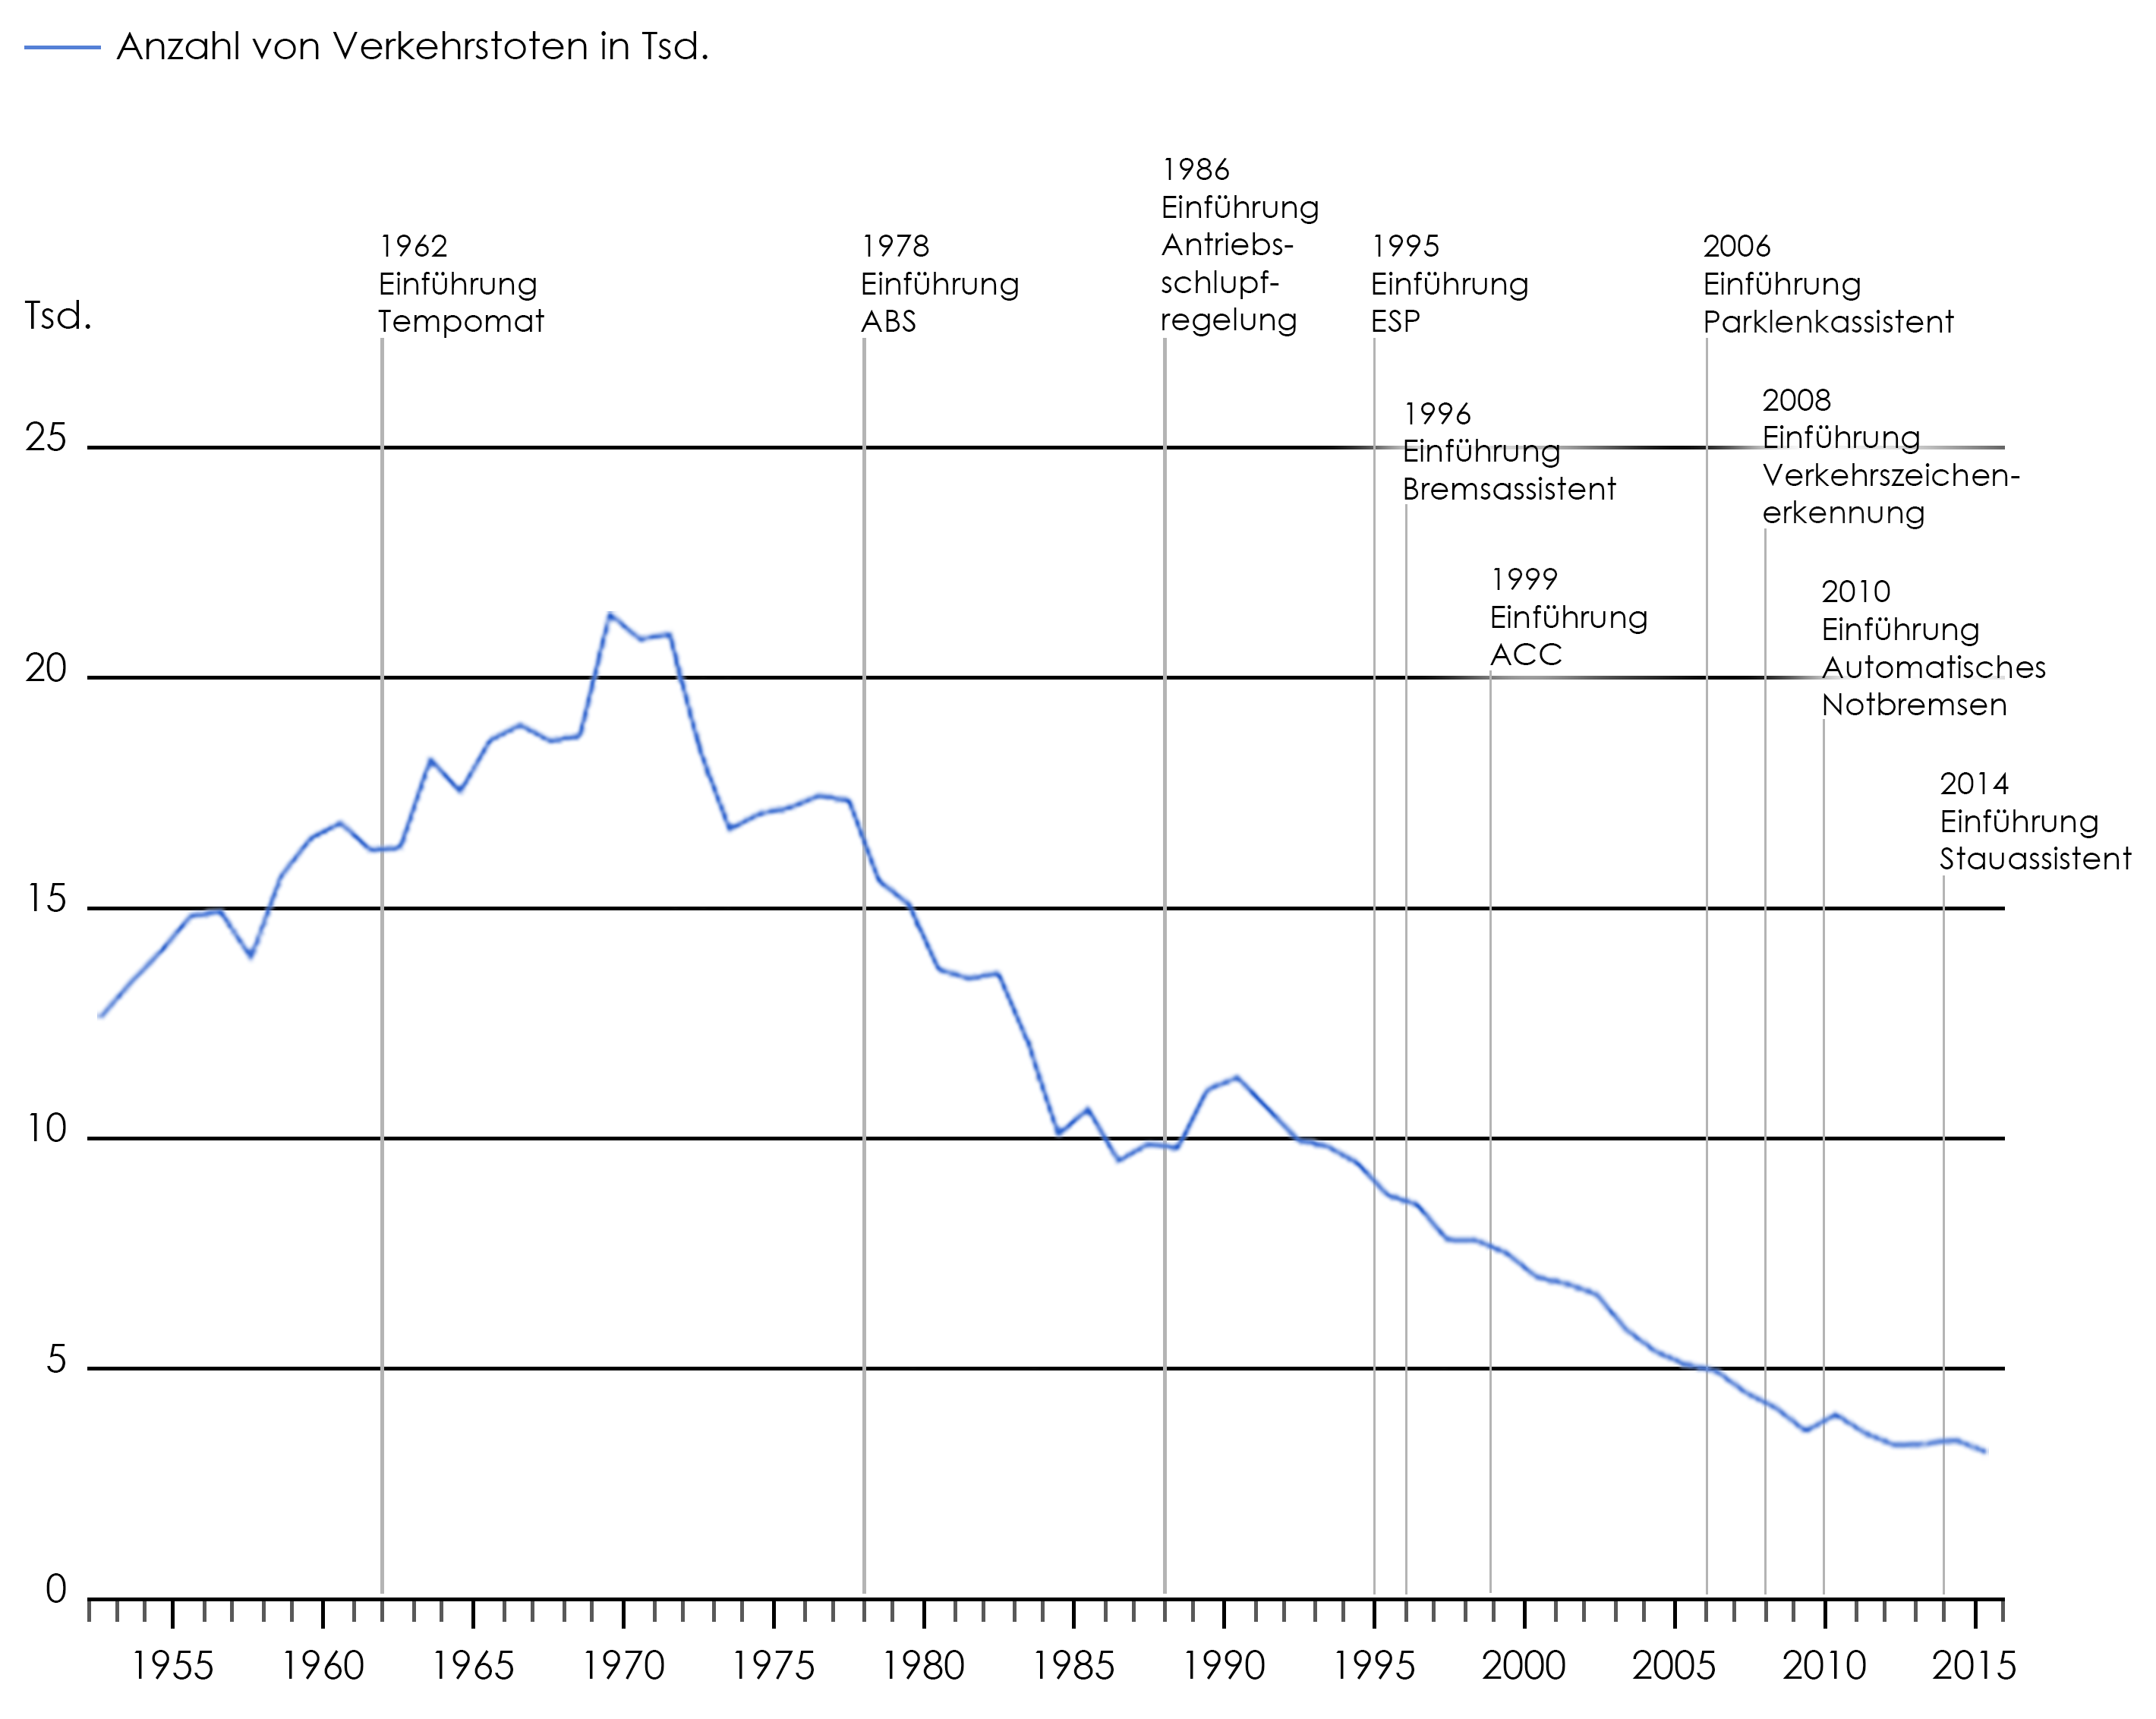
\includegraphics[width= 0.95\textwidth]{images/statistik1}
	\caption[Verlauf der Anzahl an Todesopfer im deutschen Straßenverkehr von 1953 bis 2016 in Kombination mit Einführung von Fahrerassistenzsystemen]{Statistik der Todesfälle im deutschen Straßenverkehr mit Einführungsdaten von FAS; Quelle: Statistisches Bundesamt \protect\cite{sba}}  
	\label{fig:sba}
\end{figure}

\subsection{Zielsetzung}
\glqq Die Automatisierung der Fahrzeugführung verändert die Anforderungen an das kognitive System des Autofahrers grundlegend. Um daraus keine Gefahren entstehen zu lassen, sind noch zahlreiche Fragen offen.\grqq{} \cite{schlott}. Schlott trifft diese Aussage um die kritischen Aspekte der hochautomatisierten Fahrt zu beleuchten und um auf mögliche Risiken hinzuweisen. 

Diese Arbeit befasst sich sowohl mit der Erhebung der technischen Grundlagen, als auch mit dem menschlichen Informationsverarbeitungsprozess. Die Erkenntnisse aus den einzelnen Bereichen werden aggregiert und miteinander verknüpft, um somit die Basis für ein umfassendes HMI-Konzept zu generieren. Dieses soll die benötigten Informationen aller Automatisierungsstufen zur Förderung des Vertrauens in das Gesamtsystem und Aufrechterhaltung des Situationsbewussteins darstellt, um den Fahrer zu unterstützen. 

Das auszuarbeitende Konzept soll in einem Entwicklungsfahrzeug, weitere Details siehe \autoref{sec:entfahr}, eingesetzt werden und umfasst somit nur die Automatisierungsstufen 0 bis 3, da zum aktuellen Zeitpunkt noch keine aktiven Fahrerassistenzsysteme für höhere Automatisierungsstufen zur Verfügung stehen. Dazu wird folgende Forschungsfrage gestellt: \\

\begin{tabular}{p{0.3cm} p{0.5cm} p{13cm} p{0.5cm}}
	& \textbf{RQ}	& Können die bla bla? & \\
\end{tabular}
\vspace{1em} 

Es wird angenommen, dass sich das Informationsbedürfnis des Fahrers über die Automatisierungsstufen unterschiedlich verhält und eine sich dynamisch veränderbare Anzeige gefordert wird. Daraus lassen sich folgende Hypothesen ableiten: \\

\begin{longtable}{p{0.3cm} p{0.5cm} p{13cm} p{0.5cm}}
	& \textbf{H1}	& Je höher, desto geringer. & \\
	& & & \\
	& \textbf{H2}	& Bla bla, bla bla. & \\
	& & & \\
	& \textbf{H3}	& Bla bla, bla bla. & \\
\end{longtable}			% 1. Einleitung/Introduction and problem statement
\newpage

\thispagestyle{myPageStyle}
% Kapitel 2 - Related Work / Literaturanalyse
\section{Verwandte Arbeiten}\label{sec:RelatedWork}

Lorem ipsum Lorem ipsum.

%-------------------------------------------------------------------------------------------------------------------------------------------------------------

\subsection{Research direction 1} \label{sec:rw_dir1}
Riener \cite{riener} hat sich die Frage gestellt, was sich aus dem Einsatz von Autopilotensystemen in der Luftfahrt für den Bereich des (teil)automatisierten Fahrens in der Automobilindustrie übertragen/lernen lässt und was man für die Gestaltung der Interaktion übertragbar machen könnte. usw. usw.
Gold et al. thematisierten die Frage, ``zu welchem Zeitpunkt, vor dem Auftreten einer Systemgrenze, muss das FAS die Aufmerksamkeit des Fahrers auf sich ziehen, um eine erfolgreiche Übernahme durch den Fahrer auch dann sicherzustellen, wenn er sich nicht im Loop befindet.'' \cite{gold} %
Hierzu wurde eine Studie mit 32 Probanden in einem High-Fidelity-Fahrsimulator bei BMW durchgeführt. Das Szenario beschreibt eine Fahrt mit 120 km/h auf einer dreispurigen Autobahn, bei der das vorausfahrende Auto einen Unfall verursacht und somit den Fahrer zu handeln zwingt. 17 Probanden haben dieses Szenario als Referenz manuell durchfahren, wobei der Unfall zum Einen fünf Sekunden, zum Anderen 7 Sekunden entfernt war. Die gleichen Zeiten wurden für die Probanden der hochautomatisierten Zeit eingehalten um die Übergabe einzuleiten.  

Folgende Ergebnisse konnten aus dieser Studie gezogen werden:
\begin{itemize}
	\item[1.] Die geringe Zeit bis zur Übernahme lässt die Probanden schneller zu einer Entscheidung und Reaktion kommen, dennoch ist deren Qualität schlecht.
	\item[2.] Mit der sich verringernden Zeit bis zur Übernahme nehmen die Kontrollblicke in Spiegel und über die Schulter ab, hingegen nimmt die Beschleunigung zu, sowie auch das Betätigen der Bremse.
	\item[3.] Vergleicht man die Probanden aus der Referenzfahrt und der hochautomatisierten Fahrt, wird deutlich, dass bei den Probanden der hochautomatisierten Fahrt bis zu dreimal so hohe Beschleunigungen erzielt wurden. Auch werden hier viele plötzliche Bremsmanöver durchgeführt. 
\end{itemize}

Die Studie belegt unter diesen experimentellen Bedingungen, dass bei vollständiger Ablenkung des Fahrers bei hochautomatisierter Fahrt noch bei sieben Sekunden Übernahmezeit ein Automatisierungseffekt auftritt. Das bedeutet, dass der Fahrer durch die fahr-fremde Nebentätigkeit stark abgelenkt ist und der automatisierten Fahrt vertraut. Dies führt zu solchen Reaktionen bei unerwarteter Bekanntmachung von Übernahmen. 








\subsubsection{Relevanz für die eigene Arbeit - Direction 1}

Lorem ipsum Lorem ipsum.

%-------------------------------------------------------------------------------------------------------------------------------------------------------------

\subsection{Research direction 2} \label{sec:rw_dir2}
\cite{wintersberger} befasst sich mit einer umfassenden und klar definierten Taxonomie der zwei Hautprozesse ``handover'' und ``handback''. Er kommt zu folgender Schlussfolgerung:

\begin{itemize}
	\item[1.] Handover - von der automatisierten zur manuellen Fahrt			  
	\item[2.] Handback - von der manuellen zur automatisierten Fahrt			  
\end{itemize}


\subsubsection{Relevanz für die eigene Arbeit - Direction 2}

Lorem ipsum Lorem ipsum.


\subsection{Schlussfolgerung}
Zusammenfassung des Kapitels, Ableitung von Empfehlungen, etc. für die eigene Arbeit.

\begin{itemize}
	\item Lorem ipsum \autoref{sec:rw_dir1}.
	\item Lorem ipsum lorum ipsum \autoref{sec:rw_dir1}.
	\item Lorem ipsum \autoref{sec:rw_dir2}.
	\item ...
	\item Lorem ipsum lorem ipsum lorem ipsum\autoref{sec:rw_dir2}.
\end{itemize}			% 2. Literaturanalyse/Related work analysis
\newpage
\iffalse
\thispagestyle{myPageStyle}
\input{Chapter3/chap3}		  % 3. Implementation, Technical Setting, Prototype
\newpage

\thispagestyle{myPageStyle}
\input{Chapter4/chap4}		% 4. ...
\newpage

\thispagestyle{myPageStyle}
\input{Chapter5/chap5}			% 5. ...
\newpage

\thispagestyle{myPageStyle}
\input{Chapter6/chap6}			% 6. Study design and execution
\newpage

\thispagestyle{myPageStyle}
\input{Chapter7/chap7}			% 7. Evaluation and Results
\newpage
\fi

\thispagestyle{myPageStyle}
% Kapitel 8 - Diskussion
\section{Diskussion}
Diskussion der Resultate im Vergleich zu Ergebnissen der Related work-Analyse und Reflektion auf die Forschungsfragen/Hypothesen.

Hypothese \textbf{H1} kann angenommen werden. Bla bla Begründung/Argumentation.

Andererseits zeigen die Ergebnisse der Evaluation aber keinen signifikanten Unterschied (siehe \cite{field}) zwischen X und Y - somit kann auch \textbf{H2} angenommen werden. Da hier bla bla Argumentation.

Durch die Ergebnisse des Fragebogens wird Hypothese \textbf{H3} nicht bestätigt. Es sind keine signifikanten Unterschiede über die ... 


			% 8. Discussion, Deriving concrete action recommendations
\newpage

\thispagestyle{myPageStyle}	% 9. Conclusion, Future work, Limitations
% Kapitel 9 - Fazit
\section{Fazit}
Diese Arbeit befasste sich grundsätzlich mit der Frage, welche Anforderungen an ... gestellt werden.
Der Lösungsvorschlag war...
Benutzerstudien haben gezeigt, dass es einen signifikanten Unterschied... gibt. Diese Ergebnisse motivieren, um ...

\subsection{Ausblick} 
In dieser Arbeit haben wir uns mit ... beschäftigt. Durch zwei Benutzerstudien wurde festgestellt, dass sich die Aufteilung und Positionierung der Informationen innerhalb der Anzeige der beiden Gruppen aufgrund bla bla ändert. Das entwickelte Konzept ist zwar bla bla, müsste aber für eine Wiederholung der Studien bla bla zur Erhebung quantitativer Daten wie folgt angepasst werden:

\begin{itemize}
\item xxx
\item yyy
\item xzz
\end{itemize}

Des Weiteren wurde festgestellt, dass bla bla. Auch das müssten zukünftige Varianten besser berücksichtigen, z.\,B., indem sie bla bla. Für Studien sollte zudem eine neutrale(re) Umgebung gewählt werden. Somit sollte sichergestellt werden können, dass beispielsweise ein möglicher Bias der Marke des Fahrzeugs sich nicht auf das HMI-Konzept auswirkt...

\subsection{Einschränkungen}
Hinsichtlich Einschränkungen, die eine breite Anwendung der Ergebnisse verhindern, sind zwei getrennte Bereiche zu betrachten. Zum einen die Evaluation, welche sich nur auf den ersten Teil der Arbeit bezieht, zum anderen das ausgearbeitete Konzept für die Anzeige, das auf dem ersten Teil der Arbeit aufbaut. \\ [-2.5em]

\paragraph{Evaluation} 
Bla bla.

\paragraph{Konzept}
Bla bla. Das wurde etwa in beschrieben...

%\input{chap9x} %chap9_futurework_limitations}
\newpage	

	%\shorthandon{"}
	
%--------------------------------------------------------------------------------
%-----Anhang---------------------------------------------------------------------
%--------------------------------------------------------------------------------
	
	\pagenumbering{Roman} 					% Römische Nummerierung der Kapitel/Roman page numbering
	\setcounter{page}{6} 						% Beginn bei Seitenzahl X (hier: 6) um bei oberer Nummerierung aufzuschließen/Adapt page numbering
	
	%Glossar/Glossary
	\thispagestyle{myPageStyle}
	\glssetwidest{A D A S} 						% gleicher Abstand zur 2. Spalte (längstes Wort)					
	\setglossarystyle{alttree}																	
	%\printglossary[title=Abkürzungsverzeichnis,toctitle=Abkürzungsverzeichnis] 	% Rename for German thesis
	\cleardoublepage
		
	
	%Literaturliste/Literature references
	\thispagestyle{myPageStyle}
	\bibliographystyle{plainnat}
	%\bibliographystyle{abbrv}% changed abbrvdin to abbrv % DIN-Norm für Literaturdarstellung  plaindin 
	%\bibliographystyle{abbrvnat}
	\setcitestyle{authoryear, open={(}, close={)}}
	
	\renewcommand{\refname}{Literature references} % Remove for German thesis
	\bibliography{literature}					% Pfad und Datei der Literaturdatenbank/Path and file name of literature references
	\cleardoublepage	
	
	%Anhänge/Appendices
	%\thispagestyle{myPageStyle} 
	%%----------Anhang/Appendices--------------------------------------------------------------

\appendix
\section{Anhang}

\subsection[]{Onlinefragebogen} \label{sec:a1} 
%\vspace{2em}
%\includepdf[pages={2-3}]{images/fragebogen/questionnaire2}

\subsection[]{Rohdaten des Onlinefragebogens für die statistische Auswertung}

\subsection[]{Auswertung der Evaluation hinsichtlich...}

\subsection[]{Datenträger/Data carrier}
	%\cleardoublepage
	
%----------------------------------------------------------------------------------
%----------------DOKUMENTENENDE - END OF DOCUMENT----------------------------------
%----------------------------------------------------------------------------------
	
\end{document}
